\section{Regulator PI z odsprzęganiem}
\indent Pierwszy otrzymany regulator z odsprzęganiem działał dużo gorzej od regulatora PID. Wynikało, to głownie z faktu, że bloki odsprzęgające są jak niżej zaprezentowano elementem liniowym lub w przybliżeniu linowym (czyli ich stosunek tez był liniowy, gdy jedna z wartości osiągała wartość 0). Toteż gdy sygnały z regulatorów były przycinane tak jak dla regulatora bez odsprzęgania regulator nie był w stanie osiągnąć temperatury wyższej niż w punkcie pracy. Rozwiązaniem tego problemu było wprowadzenie ograniczenia ujemnego dla sygnałów wyjściowych z regulatora i wprowadzenie minimalnej wartości sygnalu sterowania 0 dopiero po z sumowaniu sygnału z regulatora z sygnałem z bloku odsprzęgającego. Po tym zabiegu widać czasem pozytywny wpływ bloku odsprzęgającego na jakość regulacji.

\indent Człony odsprzęgające prezentują się następującymi równaniami:\\
\begin{equation}
    D12=-1
\end{equation}
\begin{equation}
    D21=\frac{0.00619z+2.122e-5}{0.002301z+7.897e-6}=~2.69
\end{equation}

\indent Transmitancja $D21$ sprowadza się do równania różnicowego:
\begin{equation}
    y(k)=\frac{7.897e-6y(k-1)+0.00619u(k)++2.122e-5u(k-1)}{0.002301}
\end{equation}

 W przypadku członu odsprzęgającego $D21$ zbadano zarówno odsprzęganie w przybliżonej formie  po wyzerowaniu składowych bliskich zeru) jak i wyrażone za pomocą równania różnicowego. Różnice były niezauważalne, na wykresach zostały przedstawione regulatory przy użyciu bardziej zaawansowanej formy.

\subsection{Dobrane nastawy regulatora PI}
\indent Parametry regulatora zostały dobrane w ten sam sposób co dla regulatora bez odsprzęgania. Również zostały zastosowane takie same ograniczenia na maksymalną wartość na maksymalną wartość sterowania oraz ten sam algorytm anti-windup. Minimalna wartość sterowania jest równa maksymalnej maksymalnej pomnożonej przez minus jeden. Przycinanie sygnałów jest również zrealizowana na wyjściu członów odsprzęgających.\\
\indent Dobrane parametry są następujące: \\
$KpFh=0.04$   $KiFh= 0.0004$ \\
$KpFcin= 0$  $ KiFcin2=-0.01$ \\



\subsection{PI dla przykładowych przebiegów z obiektem nielinowym}
\indent Największą zaletą jaką widać po wprowadzeniu bloku odsprzegania jest fakt, że uklad jest bardziej odporny na zadanie wartości skrajnej, jak w tym wypadku temperatury bliskiej minimalnej. Regulator już nie próbuję usunąć uchybu ustalonego i układ się stabilizuje.  \\
\indent Negatywnym zjawiskiem jest przypadek gdy wysokość słupa cieczy dąży do zera dla jednoczesnego wzrostu temperatury zadanej i zmniejszenia wysokości zadanej. Wynika to z faktu, że regulator próbuje zmniejszyć wysokosć słupa cieczy, ale przez odsprzęganie wyłącza oba dopływy.
% \FloatBarrier
%     \begin{figure}[h!]
   \centering
   \begin{subfigure}[b]{0.4\textwidth}
      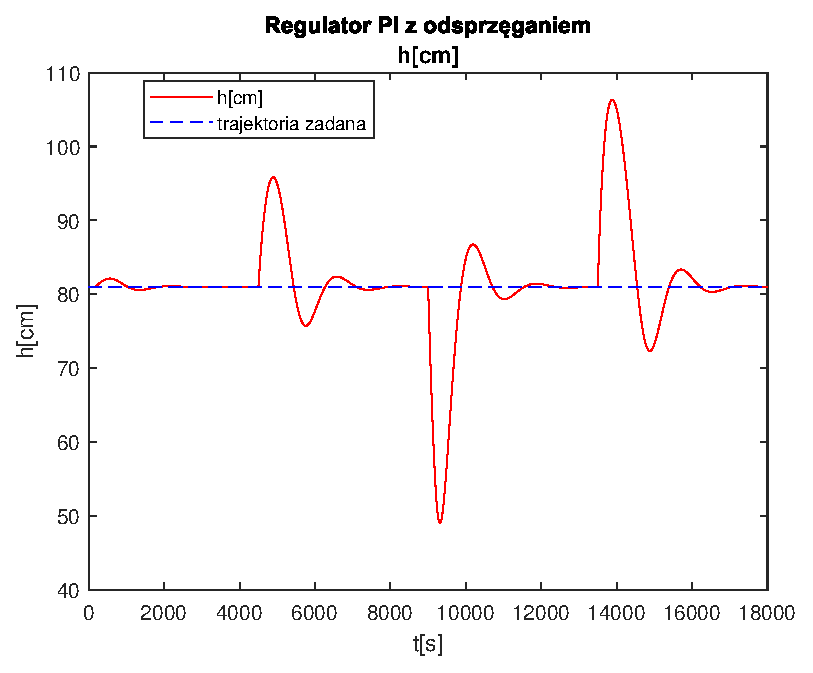
\includegraphics[width=1\linewidth]{img/PI/decoupler/disturbance/PIDecouplerH2DisttrueLinfalse.eps}
      \caption{}
      \label{fig:fig:PIDecoupler2DisttrueLinfalse1}
   \end{subfigure}
       
   \begin{subfigure}[b]{0.4\textwidth}
      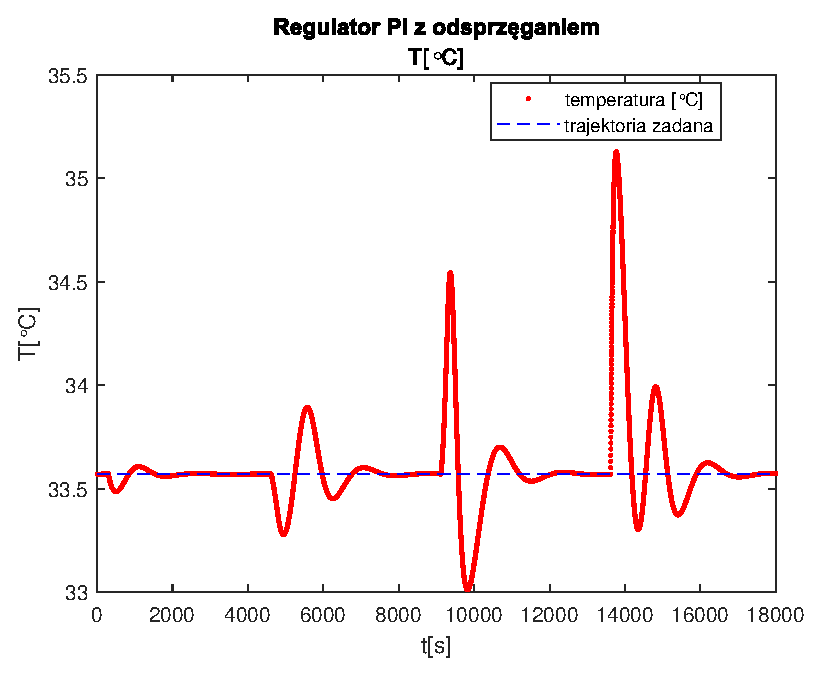
\includegraphics[width=1\linewidth]{img/PI/decoupler/disturbance/PIDecouplerT2DisttrueLinfalse.eps}
      \caption{}
      \label{fig:fig:PIDecoupler2DisttrueLinfalse2}
   \end{subfigure}
       
   \begin{subfigure}[b]{0.4\textwidth}
      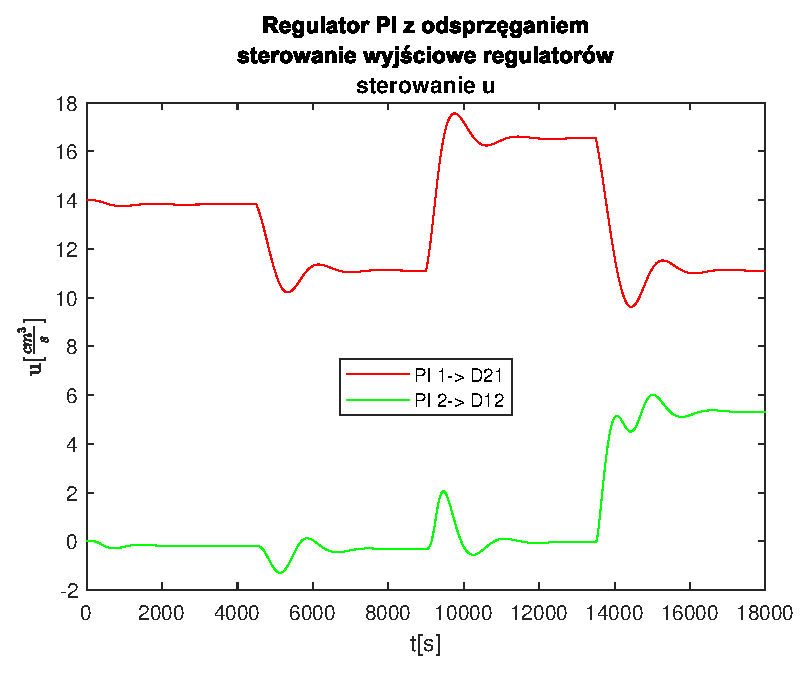
\includegraphics[width=1\linewidth]{img/PI/decoupler/disturbance/PIDecouplerControlD2DisttrueLinfalse.eps}
      \caption{}
      \label{fig:fig:PIDecoupler2DisttrueLinfalse3}
   \end{subfigure}
       
   \begin{subfigure}[b]{0.4\textwidth}
      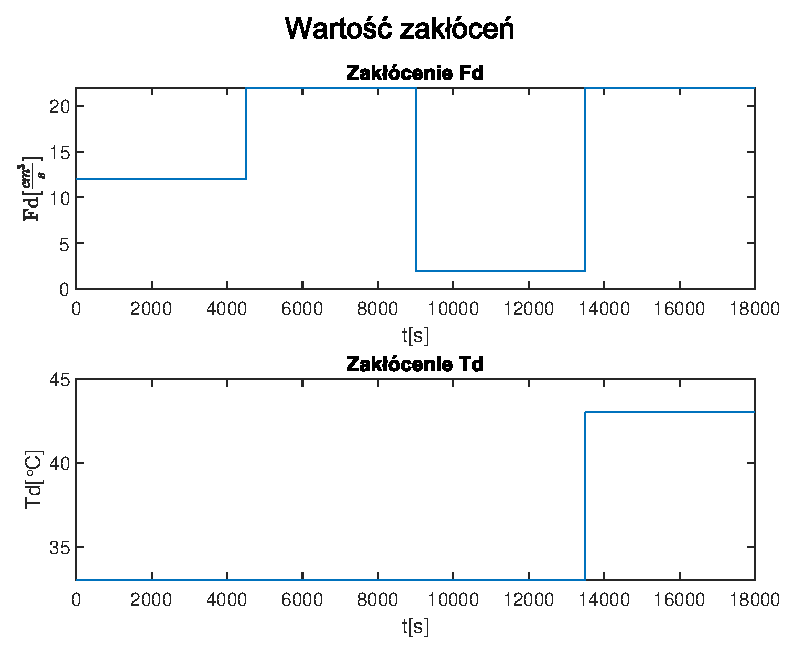
\includegraphics[width=1\linewidth]{img/PI/decoupler/disturbance/PIDecouplerDisturbance2DisttrueLinfalse.eps}
      \caption{}
      \label{fig:fig:PIDecoupler2DisttrueLinfalse4}
   \end{subfigure}
       
   \caption{Wykresy dla regulatora PI z odsprzeganiem dla różnych wartości zakłóceń}
   \label{fig:PIDecoupler2DisttrueLinfalse}
\end{figure}
           
\begin{figure}[h!]
   \centering
   \begin{subfigure}[b]{0.4\textwidth}
      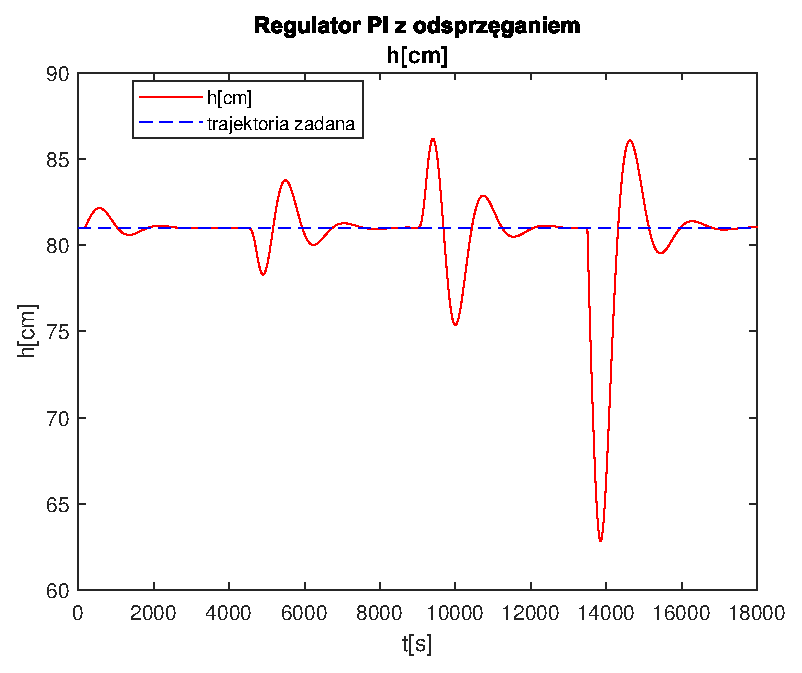
\includegraphics[width=1\linewidth]{img/PI/decoupler/disturbance/PIDecouplerH3DisttrueLinfalse.eps}
      \caption{}
      \label{fig:fig:PIDecoupler3DisttrueLinfalse1}
   \end{subfigure}
       
   \begin{subfigure}[b]{0.4\textwidth}
      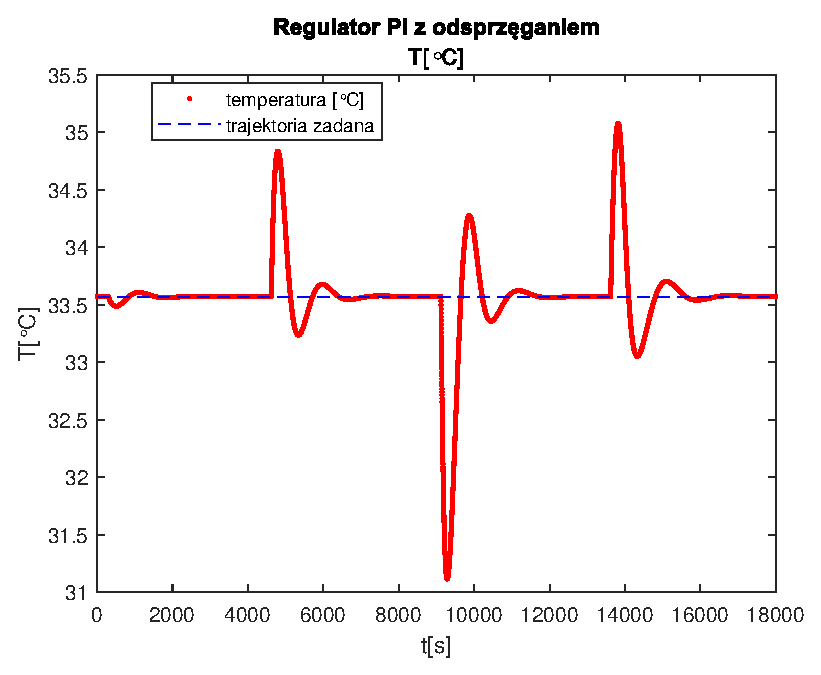
\includegraphics[width=1\linewidth]{img/PI/decoupler/disturbance/PIDecouplerT3DisttrueLinfalse.eps}
      \caption{}
      \label{fig:fig:PIDecoupler3DisttrueLinfalse2}
   \end{subfigure}
       
   \begin{subfigure}[b]{0.4\textwidth}
      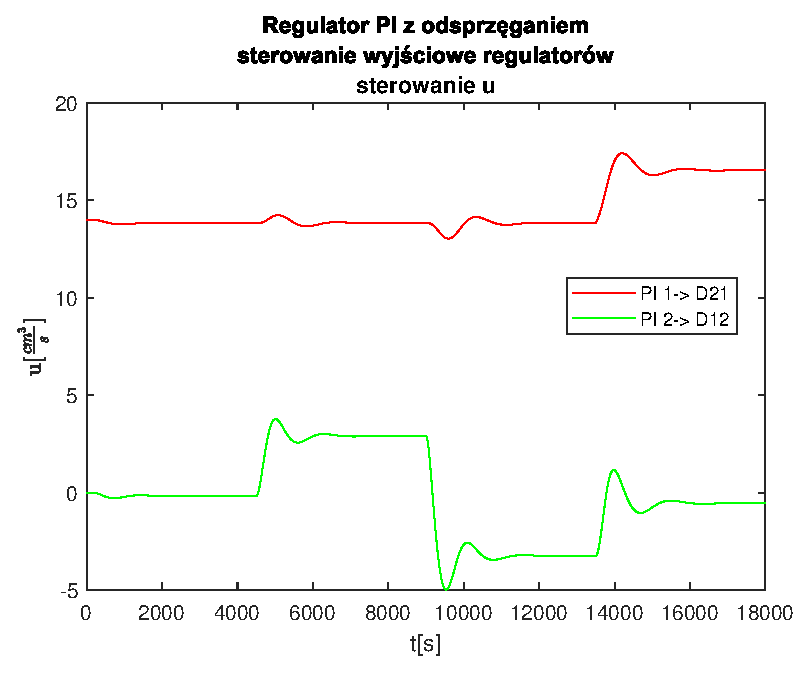
\includegraphics[width=1\linewidth]{img/PI/decoupler/disturbance/PIDecouplerControlD3DisttrueLinfalse.eps}
      \caption{}
      \label{fig:fig:PIDecoupler3DisttrueLinfalse3}
   \end{subfigure}
       
   \begin{subfigure}[b]{0.4\textwidth}
      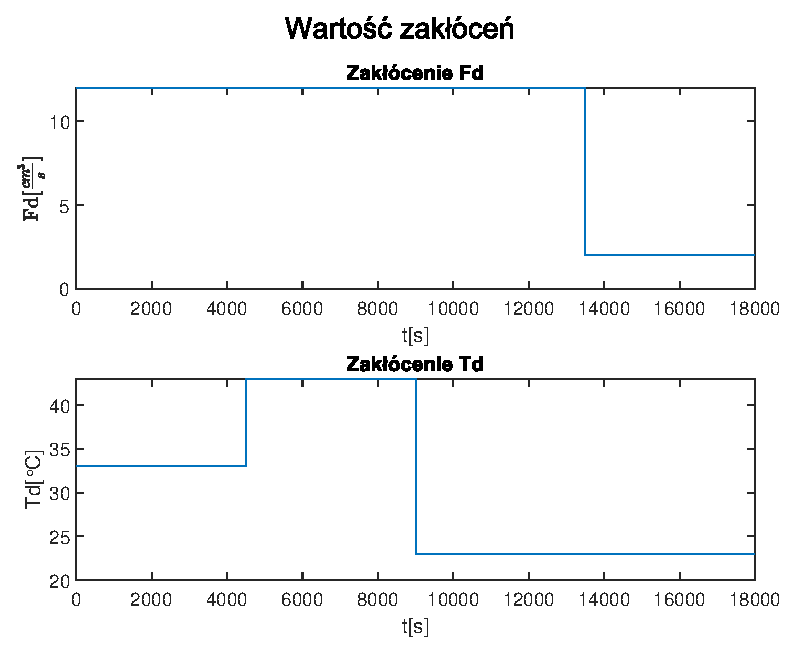
\includegraphics[width=1\linewidth]{img/PI/decoupler/disturbance/PIDecouplerDisturbance3DisttrueLinfalse.eps}
      \caption{}
      \label{fig:fig:PIDecoupler3DisttrueLinfalse4}
   \end{subfigure}
       
   \caption{Wykresy dla regulatora PI z odsprzeganiem dla różnych wartości zakłóceń}
   \label{fig:PIDecoupler3DisttrueLinfalse}
\end{figure}
           

% \FloatBarrier


\subsection{PI dla przykładowych przebiegów z obiektem zlinearyzowanym}
\indent Zostało również zbadane jak będzie się zachowywała sie symulacja gdy sterowania podamy na model zlinearyzowany. W tym wypadku zastosowanie modelu zlinearyzowanego do symulacji jest jeszcze bardziej niebezpieczne, ponieważ można osiągnąć wartość minimalną mniejszą niż jest w ogóle możliwa (temperatura mniejsza  jest od Tc w przypadku przergulowania).
\FloatBarrier
    \begin{figure}[h!]
   \centering
   \begin{subfigure}[b]{0.4\textwidth}
      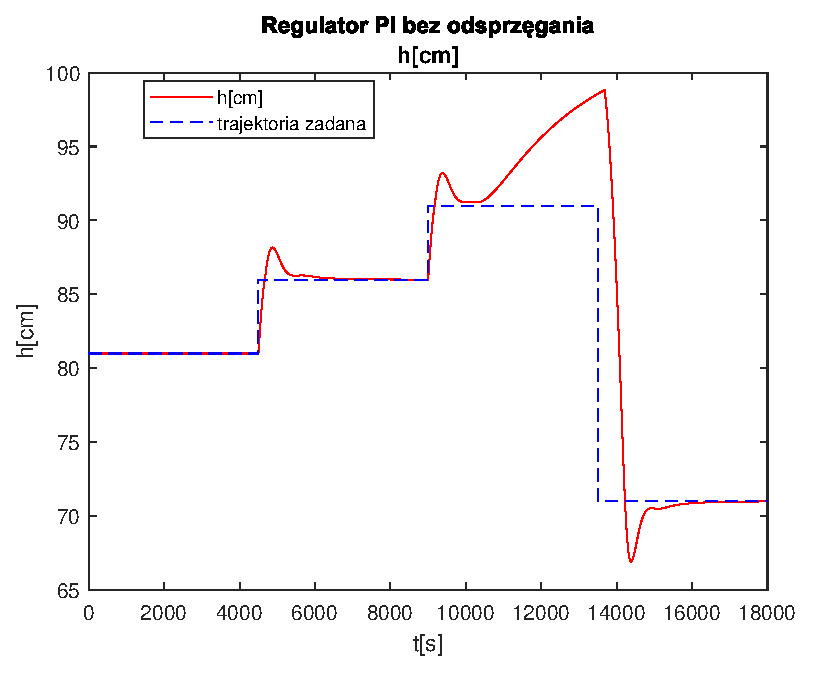
\includegraphics[width=1\linewidth]{img/PI/noDecoupler/noDisturbance/PINoDecouplerH1Lintrue.eps}
      \caption{}
      \label{fig:fig:PINodDecoupler1Lintrue1}
   \end{subfigure}
       
   \begin{subfigure}[b]{0.4\textwidth}
      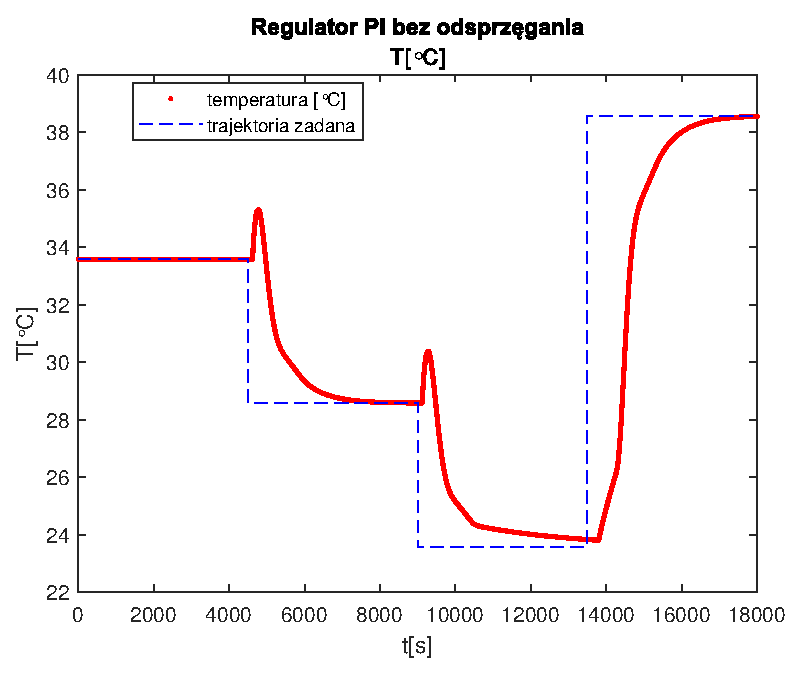
\includegraphics[width=1\linewidth]{img/PI/noDecoupler/noDisturbance/PINoDecouplerT1Lintrue.eps}
      \caption{}
      \label{fig:fig:PINodDecoupler1Lintrue2}
   \end{subfigure}
       
   \begin{subfigure}[b]{0.4\textwidth}
      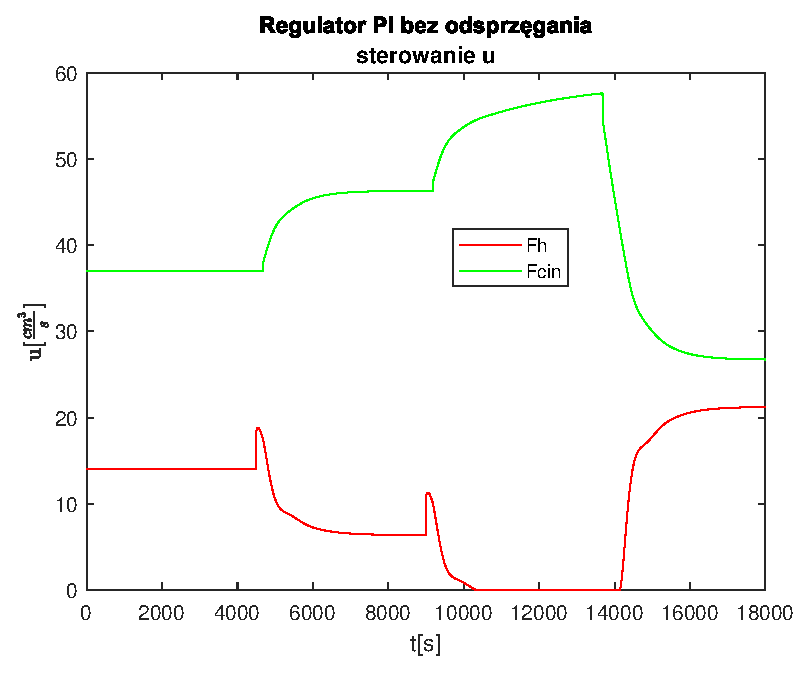
\includegraphics[width=1\linewidth]{img/PI/noDecoupler/noDisturbance/PINoDecouplerControl1Lintrue.eps}
      \caption{}
      \label{fig:fig:PINodDecoupler1Lintrue3}
   \end{subfigure}
       
   \caption{Wykresy dla regulatora PI bez odsprzegania.}
   \label{fig:PINodDecoupler1Lintrue}
\end{figure}
           
\begin{figure}[h!]
   \centering
   \begin{subfigure}[b]{0.4\textwidth}
      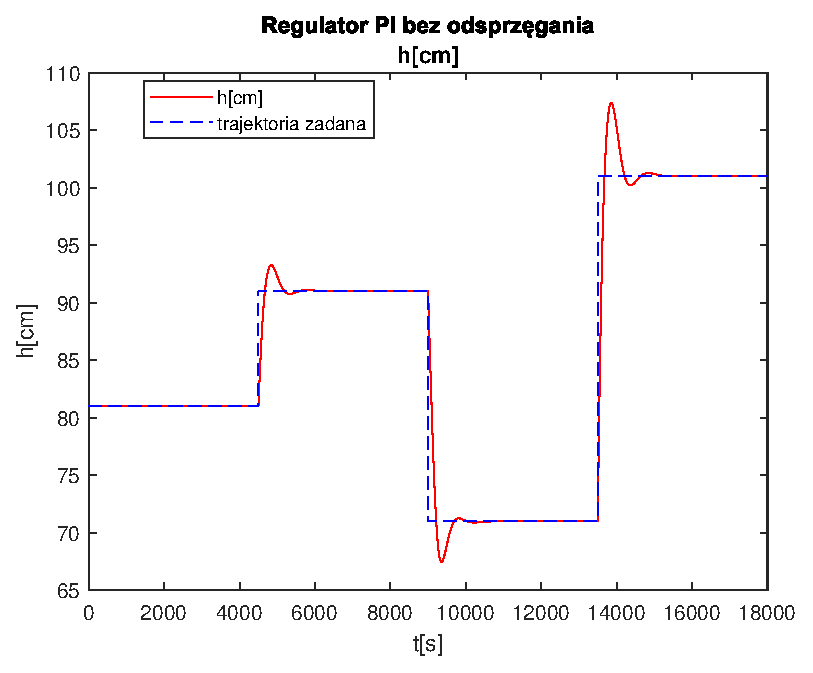
\includegraphics[width=1\linewidth]{img/PI/noDecoupler/noDisturbance/PINoDecouplerH2Lintrue.eps}
      \caption{}
      \label{fig:fig:PINodDecoupler2Lintrue1}
   \end{subfigure}
       
   \begin{subfigure}[b]{0.4\textwidth}
      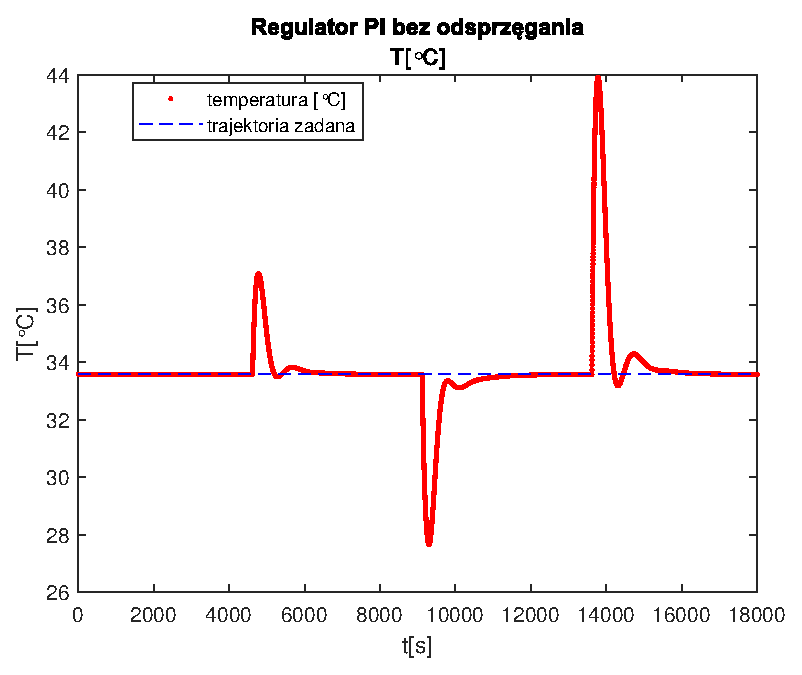
\includegraphics[width=1\linewidth]{img/PI/noDecoupler/noDisturbance/PINoDecouplerT2Lintrue.eps}
      \caption{}
      \label{fig:fig:PINodDecoupler2Lintrue2}
   \end{subfigure}
       
   \begin{subfigure}[b]{0.4\textwidth}
      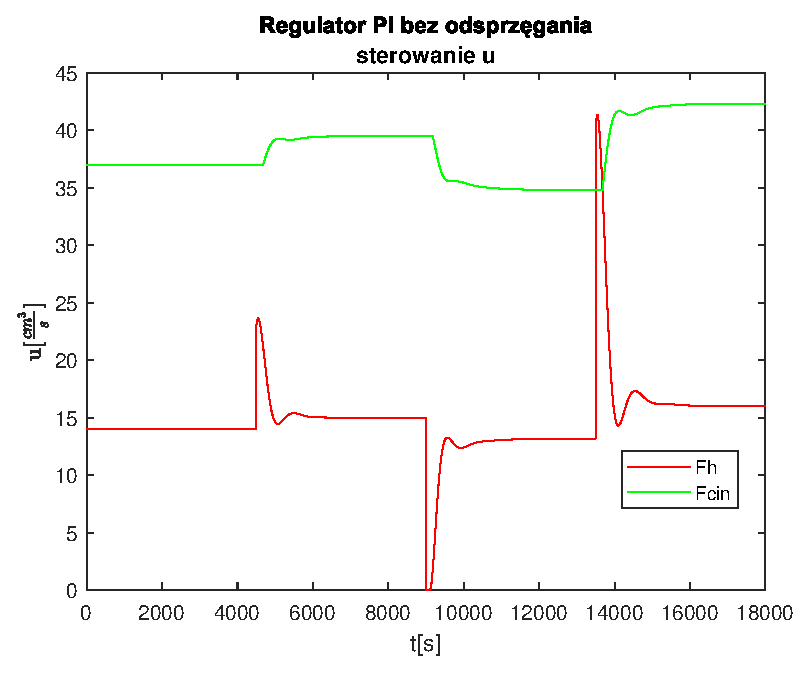
\includegraphics[width=1\linewidth]{img/PI/noDecoupler/noDisturbance/PINoDecouplerControl2Lintrue.eps}
      \caption{}
      \label{fig:fig:PINodDecoupler2Lintrue3}
   \end{subfigure}
       
   \caption{Wykresy dla regulatora PI bez odsprzegania.}
   \label{fig:PINodDecoupler2Lintrue}
\end{figure}
           
\begin{figure}[h!]
   \centering
   \begin{subfigure}[b]{0.4\textwidth}
      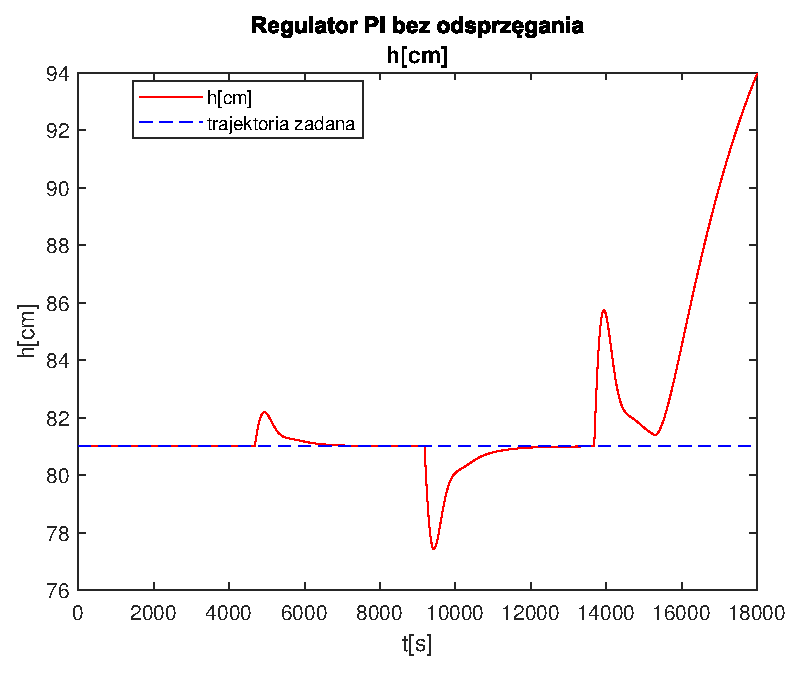
\includegraphics[width=1\linewidth]{img/PI/noDecoupler/noDisturbance/PINoDecouplerH3Lintrue.eps}
      \caption{}
      \label{fig:fig:PINodDecoupler3Lintrue1}
   \end{subfigure}
       
   \begin{subfigure}[b]{0.4\textwidth}
      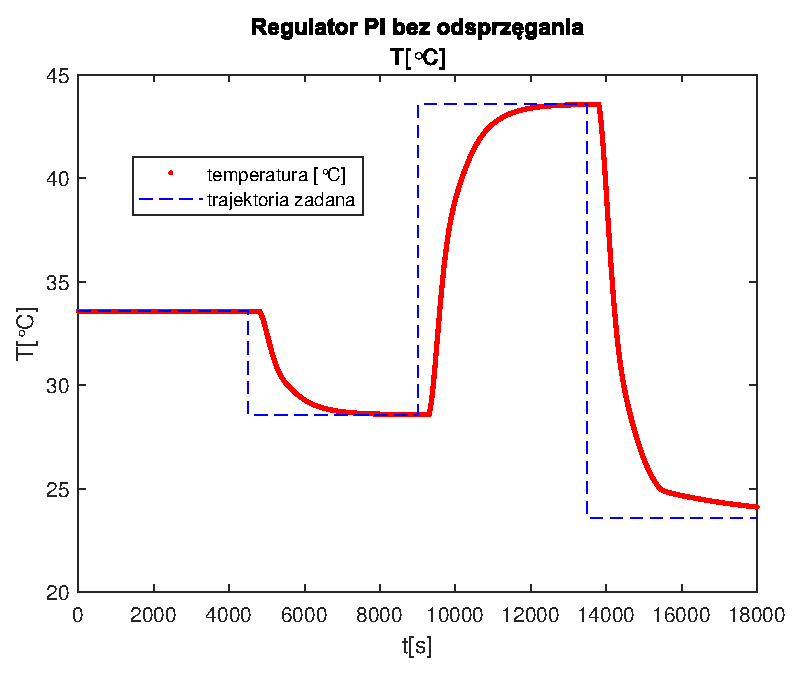
\includegraphics[width=1\linewidth]{img/PI/noDecoupler/noDisturbance/PINoDecouplerT3Lintrue.eps}
      \caption{}
      \label{fig:fig:PINodDecoupler3Lintrue2}
   \end{subfigure}
       
   \begin{subfigure}[b]{0.4\textwidth}
      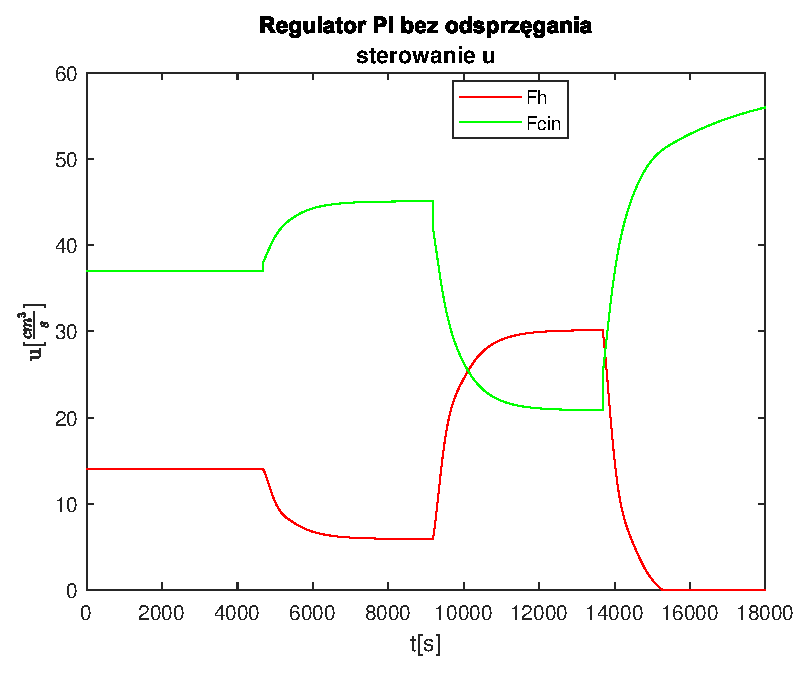
\includegraphics[width=1\linewidth]{img/PI/noDecoupler/noDisturbance/PINoDecouplerControl3Lintrue.eps}
      \caption{}
      \label{fig:fig:PINodDecoupler3Lintrue3}
   \end{subfigure}
       
   \caption{Wykresy dla regulatora PI bez odsprzegania.}
   \label{fig:PINodDecoupler3Lintrue}
\end{figure}
           

\FloatBarrier


\subsection{PI ze zmianą zakłócenia z obiektem nielinowym}
\indent Regulator radzi sobie porównywalnie z regulatorem bez odsprzęgania gdy są podane zakłócenia. Miejscami uchyby są mniejsze lub wprost minimalne. Są jednak przypadki gdy wartości uchybów są większe niż dla regulatora bez odsprzęgania.
\FloatBarrier
    \begin{figure}[h!]
   \centering
   \begin{subfigure}[b]{0.4\textwidth}
      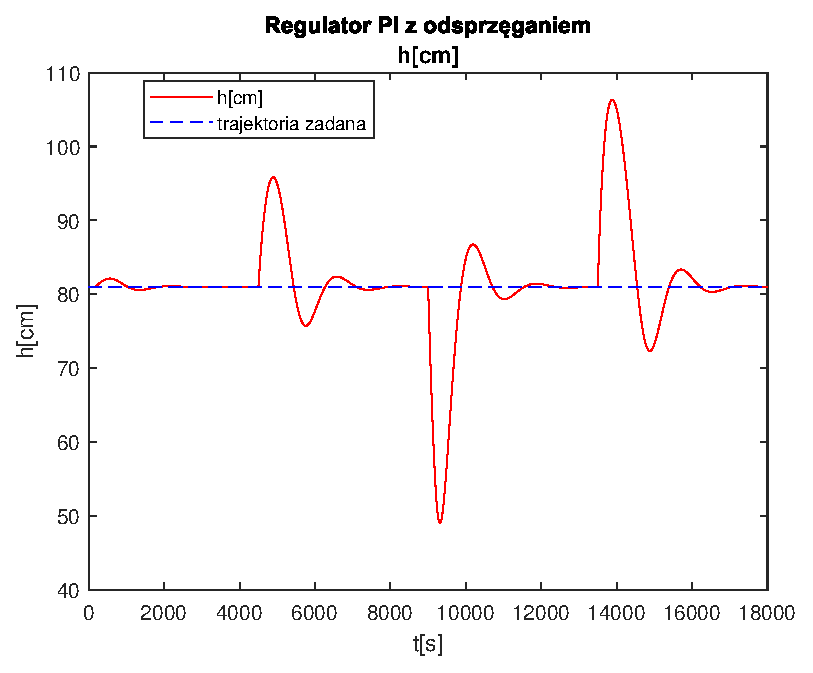
\includegraphics[width=1\linewidth]{img/PI/decoupler/disturbance/PIDecouplerH2DisttrueLinfalse.eps}
      \caption{}
      \label{fig:fig:PIDecoupler2DisttrueLinfalse1}
   \end{subfigure}
       
   \begin{subfigure}[b]{0.4\textwidth}
      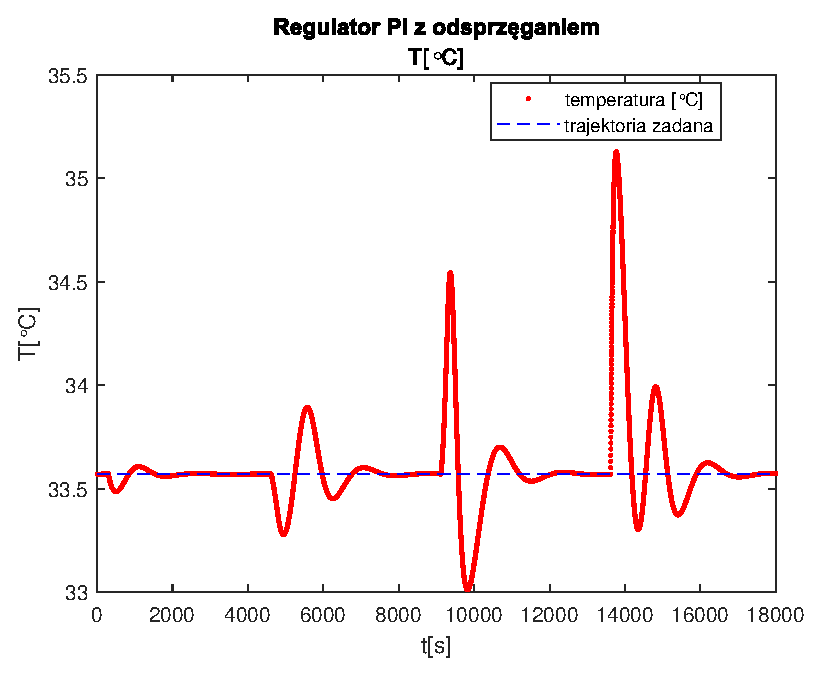
\includegraphics[width=1\linewidth]{img/PI/decoupler/disturbance/PIDecouplerT2DisttrueLinfalse.eps}
      \caption{}
      \label{fig:fig:PIDecoupler2DisttrueLinfalse2}
   \end{subfigure}
       
   \begin{subfigure}[b]{0.4\textwidth}
      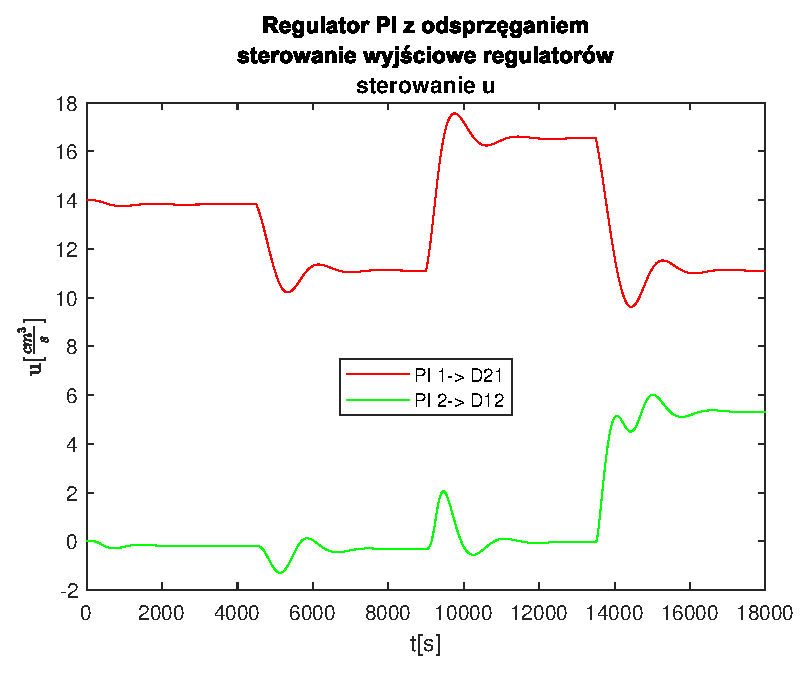
\includegraphics[width=1\linewidth]{img/PI/decoupler/disturbance/PIDecouplerControlD2DisttrueLinfalse.eps}
      \caption{}
      \label{fig:fig:PIDecoupler2DisttrueLinfalse3}
   \end{subfigure}
       
   \begin{subfigure}[b]{0.4\textwidth}
      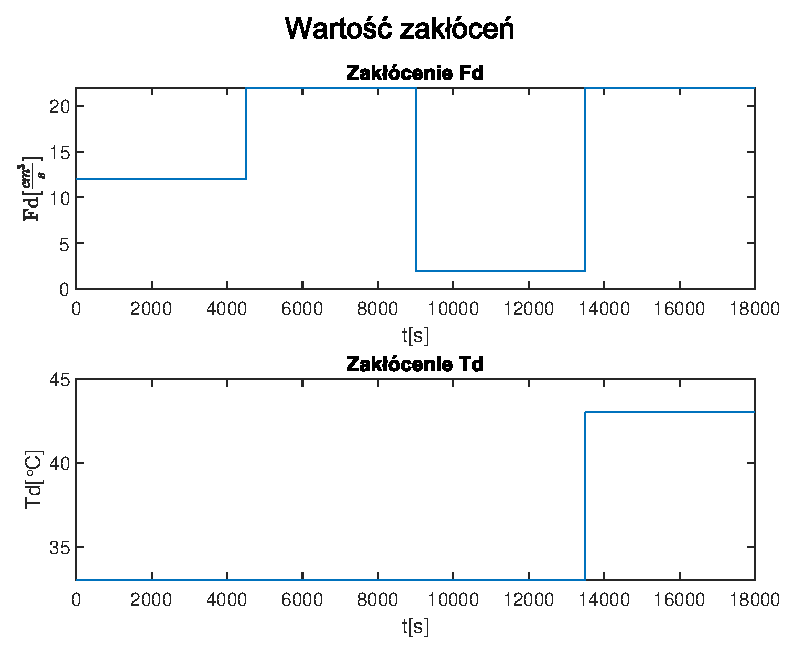
\includegraphics[width=1\linewidth]{img/PI/decoupler/disturbance/PIDecouplerDisturbance2DisttrueLinfalse.eps}
      \caption{}
      \label{fig:fig:PIDecoupler2DisttrueLinfalse4}
   \end{subfigure}
       
   \caption{Wykresy dla regulatora PI z odsprzeganiem dla różnych wartości zakłóceń}
   \label{fig:PIDecoupler2DisttrueLinfalse}
\end{figure}
           
\begin{figure}[h!]
   \centering
   \begin{subfigure}[b]{0.4\textwidth}
      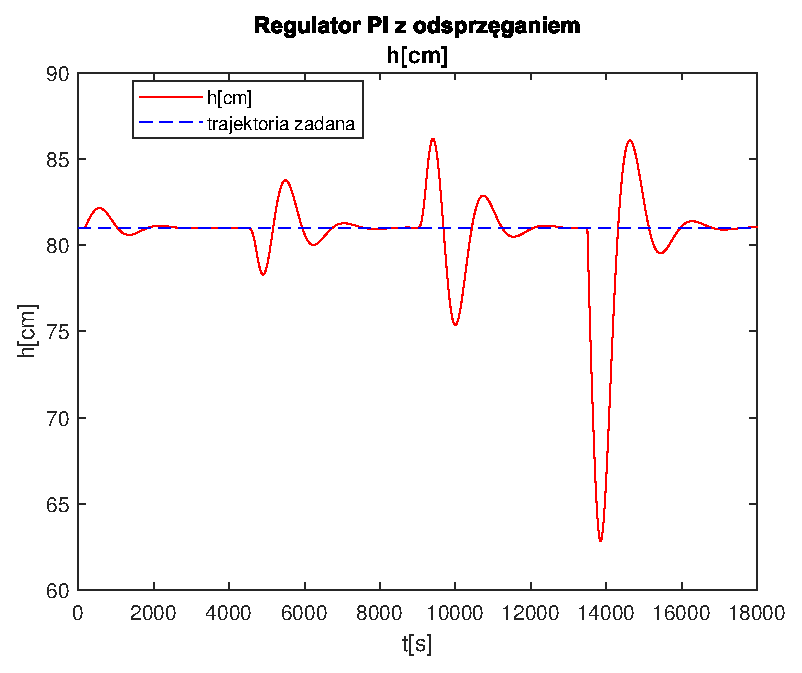
\includegraphics[width=1\linewidth]{img/PI/decoupler/disturbance/PIDecouplerH3DisttrueLinfalse.eps}
      \caption{}
      \label{fig:fig:PIDecoupler3DisttrueLinfalse1}
   \end{subfigure}
       
   \begin{subfigure}[b]{0.4\textwidth}
      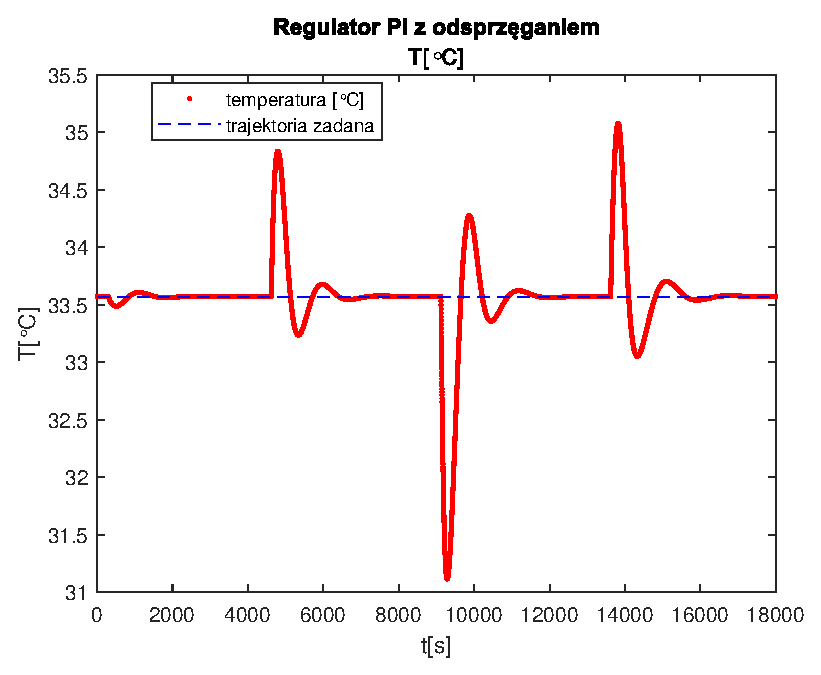
\includegraphics[width=1\linewidth]{img/PI/decoupler/disturbance/PIDecouplerT3DisttrueLinfalse.eps}
      \caption{}
      \label{fig:fig:PIDecoupler3DisttrueLinfalse2}
   \end{subfigure}
       
   \begin{subfigure}[b]{0.4\textwidth}
      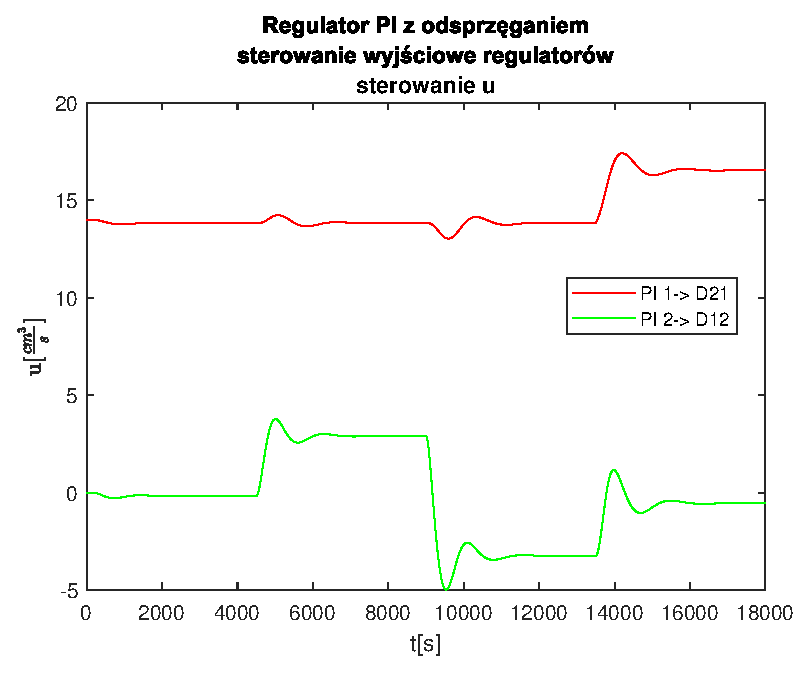
\includegraphics[width=1\linewidth]{img/PI/decoupler/disturbance/PIDecouplerControlD3DisttrueLinfalse.eps}
      \caption{}
      \label{fig:fig:PIDecoupler3DisttrueLinfalse3}
   \end{subfigure}
       
   \begin{subfigure}[b]{0.4\textwidth}
      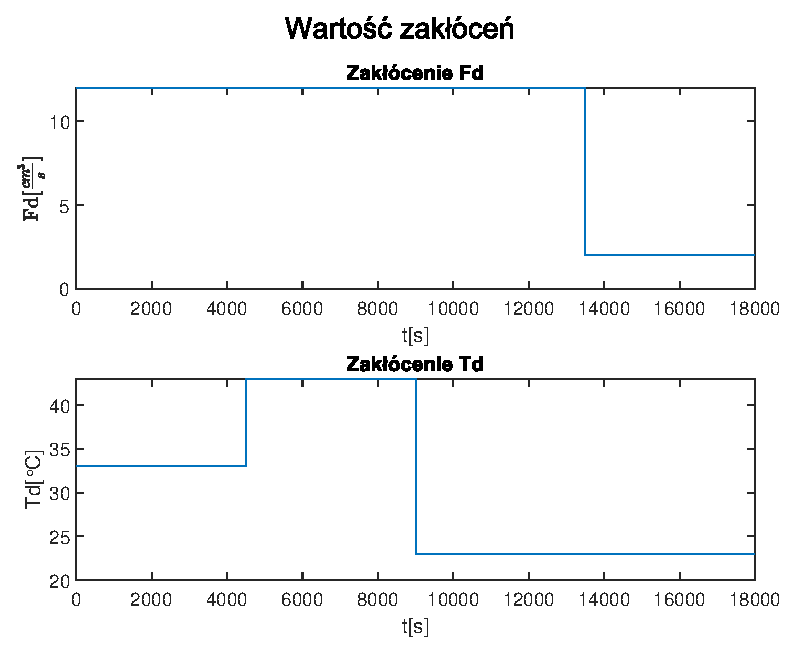
\includegraphics[width=1\linewidth]{img/PI/decoupler/disturbance/PIDecouplerDisturbance3DisttrueLinfalse.eps}
      \caption{}
      \label{fig:fig:PIDecoupler3DisttrueLinfalse4}
   \end{subfigure}
       
   \caption{Wykresy dla regulatora PI z odsprzeganiem dla różnych wartości zakłóceń}
   \label{fig:PIDecoupler3DisttrueLinfalse}
\end{figure}
           

\FloatBarrier

\subsection{Napełniania zbiornika do punktu pracy PI z modelem nieliniowym}
\indent Sprawdzając jak zachowa się układ dla napełniania zbiornika przy użyciu odprzęgania można zauważyć, że układ regulacji radzi sobie zdecydowanie lepiej niż w przypadku bez odprzęgania. Występujące prze regulowania są znikome i szybko zostają stłumione. Z charakterystyk sterowania widać, że regulator odpowiadający za dopływ zimnej wody daje na wyjściu daje wartości ujemne. Jednak człon odprzęgający koryguje tą zależność na podstawie wyliczonego dopływu ciepłej wody. Zatem charakterystyka sygnału sterującego w stanie ustalonym daję dość szybko sygnały sterujące w punkcie pracy.
\FloatBarrier
    \begin{figure}[h!]
   \centering
   \begin{subfigure}[b]{0.4\textwidth}
      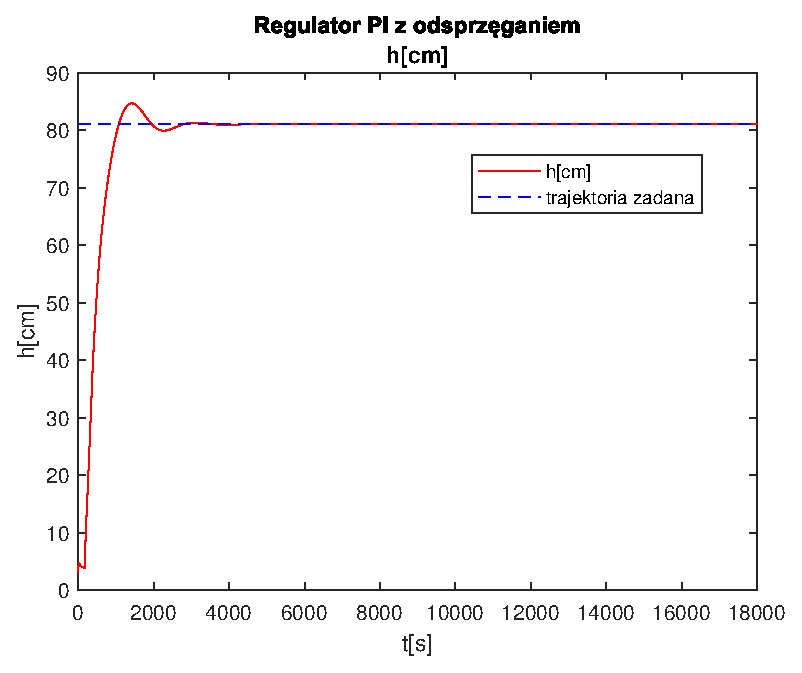
\includegraphics[width=1\linewidth]{img/PI/decoupler/noDisturbance/PIDecouplerH0.eps}
      \caption{}
      \label{fig:fig:PIDecoupler01}
   \end{subfigure}
       
   \begin{subfigure}[b]{0.4\textwidth}
      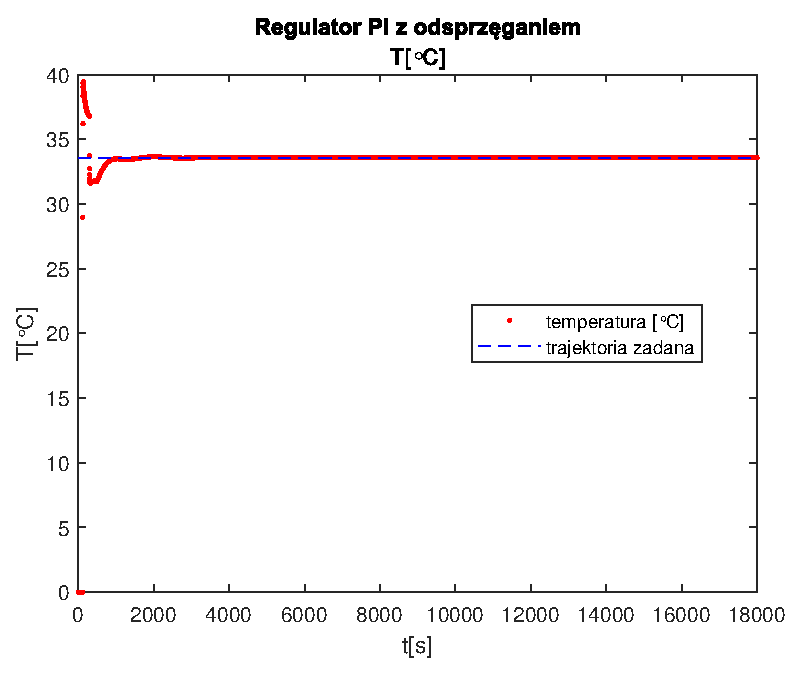
\includegraphics[width=1\linewidth]{img/PI/decoupler/noDisturbance/PIDecouplerT0.eps}
      \caption{}
      \label{fig:fig:PIDecoupler02}
   \end{subfigure}
       
   \begin{subfigure}[b]{0.4\textwidth}
      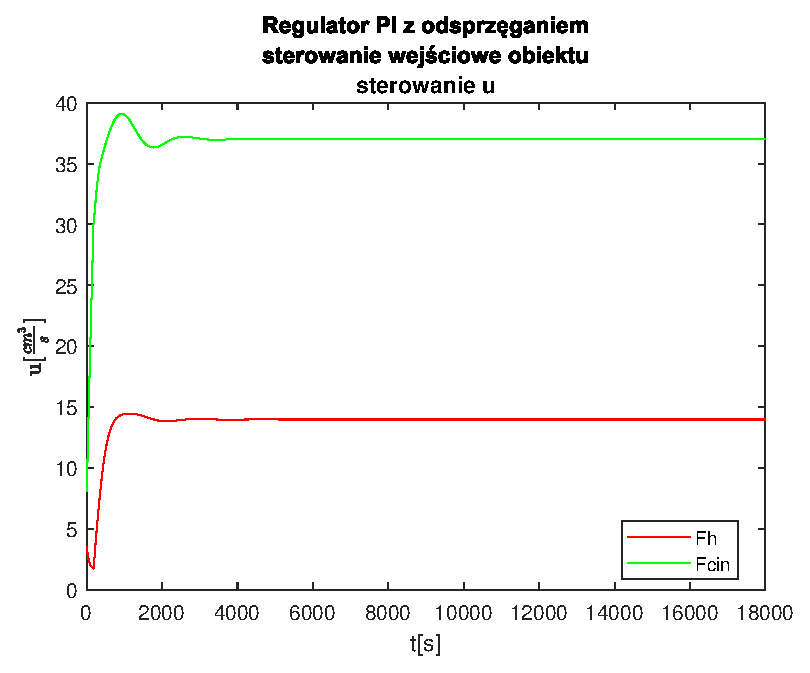
\includegraphics[width=1\linewidth]{img/PI/decoupler/noDisturbance/PIDecouplerControl0.eps}
      \caption{}
      \label{fig:fig:PIDecoupler03}
   \end{subfigure}
       
   \begin{subfigure}[b]{0.4\textwidth}
      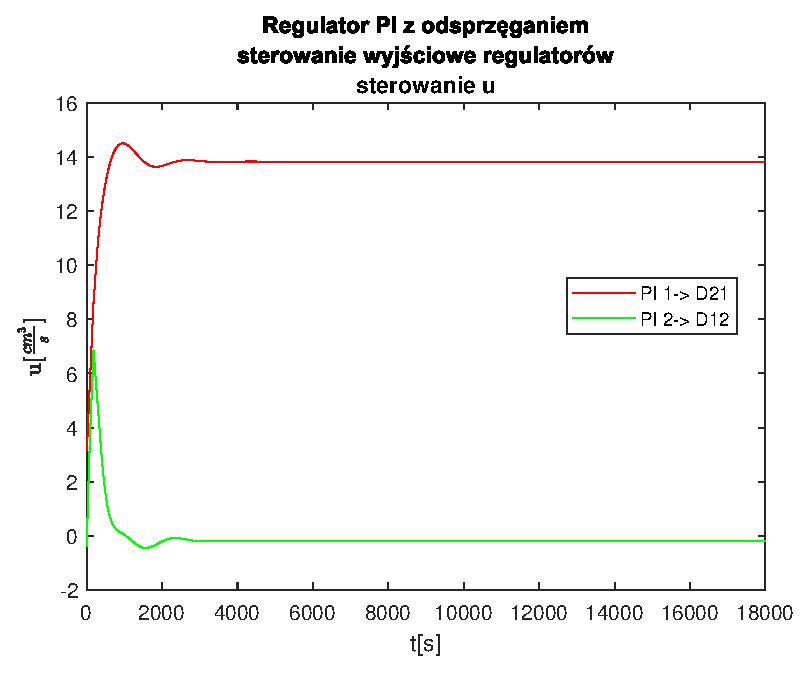
\includegraphics[width=1\linewidth]{img/PI/decoupler/noDisturbance/PIDecouplerControlD0.eps}
      \caption{}
      \label{fig:fig:PIDecoupler04}
   \end{subfigure}
       
   \caption{Wykresy dla regulatora PI z odsprzeganiem.}
   \label{fig:PIDecoupler0}
\end{figure}
           

\FloatBarrier